\begin{figure}[H]
    \centering
    \begin{subfigure}{\textwidth}
        \centering
        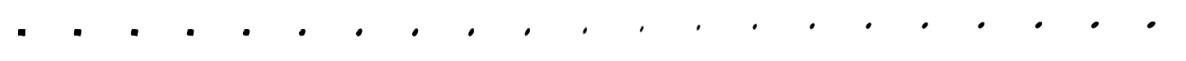
\includegraphics[width=\textwidth]{images/latent_space_entanglement/vae_7500_traverse_square_ellipse.png}
        \caption{Latent space traversal from \textit{Square} $\rightarrow$ \textit{Ellipse}}
    \end{subfigure}
    \begin{subfigure}{\textwidth}
        \centering
        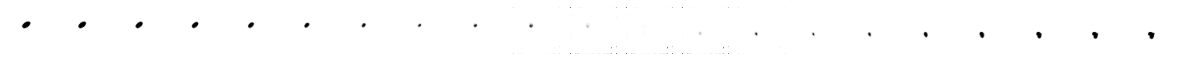
\includegraphics[width=\textwidth]{images/latent_space_entanglement/vae_7500_traverse_ellipse_heart.png}
        \caption{Latent space traversal from \textit{Ellipse} $\rightarrow$ \textit{Heart}}
    \end{subfigure}
    \begin{subfigure}{\textwidth}
        \centering
        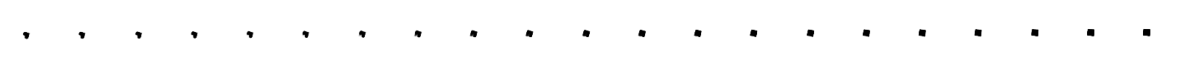
\includegraphics[width=\textwidth]{images/latent_space_entanglement/vae_7500_traverse_heart_square.png}
        \caption{Latent space traversal from \textit{Heart} $\rightarrow$ \textit{Square}}
        \label{subfig:10000_vae_latent_space_traversal_heart_to_square}
    \end{subfigure}
    \caption[7,500-VAE - Latent Space Traversal]{Latent space traversal between latent space representations of images with certain shapes for 7,500-\ac{VAE}. Color-values were inverted for this plot.}
    \label{fig:7500_vae_latent_space_traversal_shape_to_shape}
\end{figure}

\begin{figure}[H]
    \centering
    \begin{subfigure}{\textwidth}
        \centering
        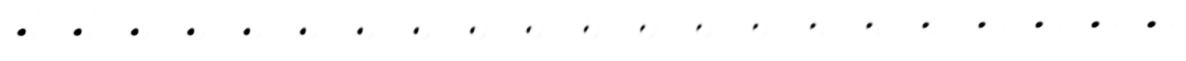
\includegraphics[width=\textwidth]{images/latent_space_entanglement/vae_5000_traverse_square_ellipse.png}
        \caption{Latent space traversal from \textit{Square} $\rightarrow$ \textit{Ellipse}}
    \end{subfigure}
    \begin{subfigure}{\textwidth}
        \centering
        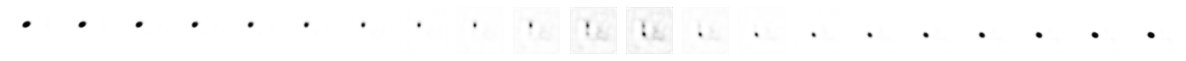
\includegraphics[width=\textwidth]{images/latent_space_entanglement/vae_5000_traverse_ellipse_heart.png}
        \caption{Latent space traversal from \textit{Ellipse} $\rightarrow$ \textit{Heart}}
    \end{subfigure}
    \begin{subfigure}{\textwidth}
        \centering
        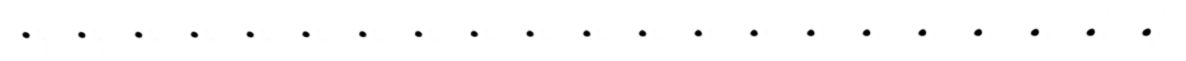
\includegraphics[width=\textwidth]{images/latent_space_entanglement/vae_5000_traverse_heart_square.png}
        \caption{Latent space traversal from \textit{Heart} $\rightarrow$ \textit{Square}}
        \label{subfig:10000_vae_latent_space_traversal_heart_to_square}
    \end{subfigure}
    \caption[5,000-VAE - Latent Space Traversal]{Latent space traversal between latent space representations of images with certain shapes for 5,000-\ac{VAE}. Color-values were inverted for this plot.}
    \label{fig:5000_vae_latent_space_traversal_shape_to_shape}
\end{figure}